\documentclass[a4paper,11pt,fleqn]{article}%fleqn pour aligner les equations à gauche
\usepackage{graphicx}
\usepackage[utf8]{inputenc}  
\usepackage[T1]{fontenc}
\usepackage{lscape}

\usepackage{tgheros,textcomp}%Police Arial
\renewcommand{\familydefault}{\sfdefault}

%\setlength{\mathindent}{0pt}%indentation dans math = 0

\usepackage[top = 1cm, bottom = 2cm, left = 1cm, right = 1cm]{geometry}
\usepackage{titlesec}
%\setcounter{secnumdepth}{4}
\usepackage{xcolor}
\usepackage{amssymb} %double flèche de réaction
\usepackage{mathrsfs}%farraday
\usepackage{xtab}%tableau sur plusieurs pages
\usepackage{esvect}%grands vecteurs

\usepackage[version=4]{mhchem} %equations chimiques

\usepackage{array}
\usepackage{chemfig}
\usepackage{multirow}
%\usepackage{sectsty}

\usepackage{caption}
\usepackage{adjustbox}
\usepackage[labelformat=simple]{subfig}
\usepackage{float}


\usepackage{amsmath}
\usepackage{amssymb}
\usepackage[cal=boondoxo]{mathalfa} 
\usepackage{enumitem}
\usepackage{lastpage}
\usepackage{tcolorbox}
\usepackage{siunitx}
\usepackage[european, straightvoltages, RPvoltages]{circuitikz}
\usepackage{tikz}
\usetikzlibrary{shapes.geometric}
\usetikzlibrary{calc}
\usetikzlibrary{automata,positioning}
\usepackage{multicol}
\usepackage{eqnarray}
\usepackage{tabularx,colortbl}%colorer fond cellules

\sisetup{
	detect-all,
	output-decimal-marker={,},
	group-minimum-digits = 3,
	group-separator={~},
	number-unit-separator={~},
	inter-unit-product={~}
} %setup pour SIunitx

\usepackage{listings}%pour insérer le code python
\definecolor{codegreen}{rgb}{0,0.6,0}
\definecolor{codegray}{rgb}{0.5,0.5,0.5}
\definecolor{codepurple}{rgb}{0.58,0,0.82}
\definecolor{backcolour}{rgb}{0.95,0.95,0.92}


%\graphicspath{ {/home/rweye/Documents/Enseignement/2023/Cours/TSPE/Eval/Ressources/} }

\titleformat{\section}
{\titlerule
\vspace{.8ex}%
\normalfont \bfseries}
{\thesection :}{.5em}{\bfseries}

\renewcommand{\thesection}{Exercice \arabic{section}}
\titlespacing{\section}{0pt}{1em}{1em}
\renewcommand{\thesubsection}{\hspace{1cm}\alph{subsection}.}
\renewcommand\thesubfigure{\textbf{Document \arabic{subfigure} :}}

\title{\vspace{-1cm}\large 
	\begin{tabular}{|m{5cm}|>{\centering}m{8cm}|>{\centering\arraybackslash}m{4cm}|}
		\hline
		Nom : & \textbf{\textsc{DS TSPE N°2}} &  Note : \\
		Prénom : & & \\\hline
\end{tabular}}
\date{}

\newpagestyle{mystyle}{%
	\setfoot{ROSALIE}{\thepage\,$|$\,\pageref{LastPage}}{}
}
\renewpagestyle{plain}{%
	\setfoot{ROSALIE}{\thepage\,$|$\,\pageref{LastPage}}{}
}

\pagestyle{mystyle}

\newenvironment{itemize*}%
{\begin{itemize}[label=$-$]%
		\setlength{\itemsep}{0pt}%
		\setlength{\parskip}{0pt}}%
	{\end{itemize}}

\newenvironment{itemize**}%
{\begin{itemize}[label=,labelindent=0pt, leftmargin=*,topsep=0pt]%
		\setlength{\itemsep}{0pt}%
		\setlength{\parskip}{0pt}}%
	{\end{itemize}}

\renewcommand{\arraystretch}{1.5}


\begin{document}
\maketitle
\vspace{-2.5cm}

\section{Coloration capillaire}
Les coloration capillaires classiques sont des solutions basiques à base d'ammoniaque. Elles sont classées en deux catégories en fonction de l'utilisation : les colorations commerciales, avec une teneur de \num{27} à \SI{30}{\percent} d'ammoniaque et les mélanges professionnels avec une teneur maximale de \SI{6}{\percent}.\\

On propose de déterminer la concentration en ammoniaque (\ce{NH3}) d'une solution servant de base pour une préparation commerciale de coloration capillaire notée $S_0$ de concentration notée $c_0$. Pour cela, on réalise un titrage sur \SI{10}{mL} de solution diluée,  grâce à une solution titrante d'acide chlorhydrique \ce{HCl} de concentration $c_A$ = \SI{1E-3}{\mole\per\liter}.

Le suivi de la réaction se fait grâce à une sonde de conductimétrie et les points mesurés sont reportés dans le graphique du document fourni.

	\subsection{Étude préliminaire}

\begin{enumerate}
	\item La solution à titrer semble trop concentrée pour un titrage direct, une  d'un facteur 10 est donc réalisé pour créer une solution titrée $S_1$ de concentration notée $c_1$. Lister le matériel nécessaire pour réaliser \SI{50}{mL} de solution $S_1$.
	\item Quelles sont les limites d'un suivi par conductimétrie ?
	\item Écrire la réaction de se produisant entre l'ammoniac \ce{NH3} et l'eau. Puis celle se produisant entre l'acide chlorhydrique \ce{HCl} et l'eau.
	\item En déduire la réaction support du titrage.
	\item Réaliser un schéma du titrage
	\item Compléter le tableau suivant en faisant figurer l'évolution de la quantité de matière de chaque espèce ionique dans le milieu au cours du titrage.
\end{enumerate}
\begin{table}[h!]
\centering
	\begin{tabular}{|>{\centering}m{0.2\textwidth}|>{\centering}m{0.15\textwidth}|>{\centering}m{0.15\textwidth}|>{\centering}m{0.15\textwidth}|>{\centering\arraybackslash}m{0.15\textwidth}|} \hline
	\textbf{Espèce ionique} & &&&\\ \hline
	\textbf{Avant équivalence} & &&&\\ \hline
	\textbf{A l'équivalence} & &&&\\ \hline
	\textbf{Après l'équivalence} & &&&\\ \hline
	\end{tabular}
\end{table}

	\subsection{Exploitation des résultats}

\begin{enumerate}[resume]
	\item En vous aidant du tableau précédent, et des valeurs de conductivité molaires ioniques fournies, justifier l'allure de la courbe de titrage.
	\item Déterminer, en explicitant la méthode employée, la valeur du volume équivalent.
	\item Calculer la valeur de la concentration $c_1$.
	\item Déterminer la valeur de la concentration de la solution de coloration capillaire.
	\item Vérifier que les valeurs obtenues sont en accord avec la teneur en ammoniaque fournie par le vendeur.
\end{enumerate}

\begin{figure}[h!]
\centering
	
\includegraphics[width = .7\textwidth]{Ressources/TSPE_DS2_Fig2.png}
\end{figure}

\begin{minipage}{.97\textwidth}
\textbf{Données : }
\begin{itemize}
	\item \textbf{Couples acide/base :} \ce{NH4+}/\ce{NH3} ; \ce{H3O+}/\ce{H2O} ; \ce{H2O}/\ce{HO-} 
	\item \textbf{Densité de la base pour coloration capillaire : }$d$ = \num{0.9}
	\item \textbf{Masse molaire de l'ammoniac : } $M$ = \SI{17}{\gram\per\mole}
	\item \textbf{Conductivités molaires ioniques : }\\
	$\lambda(\ce{NH4+})$ = \SI{7.35}{\milli\siemens\meter\squared\per\mole}\\
	$\lambda(\ce{Cl-})$ = \SI{7.63}{\milli\siemens\meter\squared\per\mole}\\
	$\lambda(\ce{HO-})$ = \SI{19.8}{\milli\siemens\meter\squared\per\mole}\\
	$\lambda(\ce{H3O+})$ = \SI{35.0}{\milli\siemens\meter\squared\per\mole}\\
\end{itemize}
\end{minipage}

\section{Lancé de marteau}
Originaire d'anciennes pratiques celtes, le lancer du marteau est une discipline de l'athlétisme qui consiste à lancer le plus loin possible un boulet auquel est fixé un câble en acier muni d'une poignée.\\
À cette fin, l'athlète fait d'abord prendre de la vitesse à son marteau en tournant sur lui-même sans sortir d'un cercle de lancement. Le marteau est ensuite lâché avec une vitesse initiale $v_0$ = \SI{26}{\meter\per\second}, avant d'atterrir sur le sol. 
	\subsection{Étude du mouvement du boulet avant le lâcher du marteau de l'athlète}
	Pour simplifier l'étude, on suppose que l'athlète tourne sur elle-même autour d'un axe immobile vertical et que son bras est toujours tendu. On notera que la longueur de son bras tendu et la chaine du marteau fait $L$ = \SI{1.5}{m}. Dans le référentiel terrestre, le mouvement du boulet est alors supposé plan et circulaire, accéléré dans un premier temps puis uniforme dans un deuxième temps.
	\begin{enumerate}
		\item A partir de la définition du vecteur accélération $\vec{a}$, montrer qu'il existe toujours une accélération lors d'un mouvement circulaire.
		\item En justifiant votre réponse, choisir parmi les schémas ci-dessous, celui qui correspond à un mouvement circulaire accéléré puis celui qui correspond à un mouvement circulaire uniforme.
	\end{enumerate}

\begin{figure}[h!]
\centering
	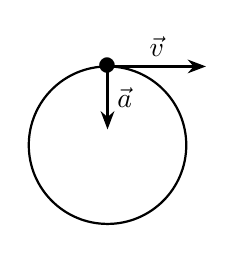
\begin{tikzpicture}
	\draw[thick] (0,0) circle(1);
	\draw[-Stealth,thick] (0,1) to (0,.2);
	\draw[-Stealth,thick] (0,1) to (1.25,1);
	\node (M1) at (0,1) {\Large $\bullet$};
	\node[right] (a1) at (0,.6) {$\vec{a}$};
	\node[above] (a1) at (.625,1) {$\vec{v}$};
	\end{tikzpicture} \hspace{1cm}
	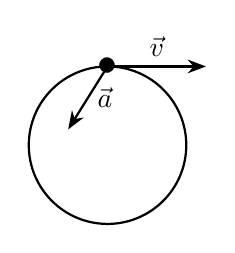
\begin{tikzpicture}
	\draw[thick] (0,0) circle(1);
	\draw[-Stealth,thick] (0,1) to (-.5,.2);
	\draw[-Stealth,thick] (0,1) to (1.25,1);
	\node (M1) at (0,1) {\Large $\bullet$};
	\node[right] (a1) at (-.25,.6) {$\vec{a}$};
	\node[above] (a1) at (.625,1) {$\vec{v}$};
	\end{tikzpicture} \hspace{1cm}
	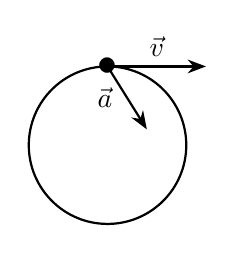
\begin{tikzpicture}
	\draw[thick] (0,0) circle(1);
	\draw[-Stealth,thick] (0,1) to (.5,.2);
	\draw[-Stealth,thick] (0,1) to (1.25,1);
	\node (M1) at (0,1) {\Large $\bullet$};
	\node[right] (a1) at (-.25,.6) {$\vec{a}$};
	\node[above] (a1) at (.625,1) {$\vec{v}$};
	\end{tikzpicture} \hspace{1cm}
	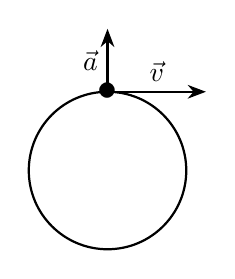
\begin{tikzpicture}
	\draw[thick] (0,0) circle(1);
	\draw[-Stealth,thick] (0,1) to (0,1.8);
	\draw[-Stealth,thick] (0,1) to (1.25,1);
	\node (M1) at (0,1) {\Large $\bullet$};
	\node[left] (a1) at (0,1.4) {$\vec{a}$};
	\node[above] (a1) at (.625,1) {$\vec{v}$};
	\end{tikzpicture}

\end{figure}
	
	\begin{enumerate}[resume]
		\item Lors de la deuxième phase du mouvement, exprimer puis calculer la norme du vecteur accélération noté $\overrightarrow{a_f}$.
	\end{enumerate}
	
	\subsection{Étude du mouvement du boulet après le lâcher du marteau}
	
	\begin{enumerate}[resume]
		\item Identifier le référentiel utilisé pour l'étude.
		\item Les équations horaires de la position du boulet sont les suivantes : 
		$$\overrightarrow{OM(t)} = \left\lbrace \begin{array}{l}
			x(t) = v_0 \cdot t \cdot \cos{45} \\
			y(t) = -\frac{1}{2} \cdot 9.81\cdot t^2+v_0 \cdot t \cdot \sin{45} +1.5 \\
		\end{array} \right\rbrace_{(O,\vec{i},\vec{j})}$$
		En se basant sur les expressions ci-dessus réaliser un schéma sans soucis d'échelle de la situation à $t=0$.
		\item Déterminer le temps mis par le boulet pour toucher le sol, à partir de l'expression de $y(t)$.
		\item Calculer la distance séparant la lanceuse et le point d'impact au sol.
		\item Déterminer les expressions de $v_x(t)$ et $v_y(t)$ en détaillant la méthode utilisée.
		\item Déterminer les expressions de $a_x(t)$ et $a_y(t)$ en détaillant la méthode utilisée.
		\item Décrire le mouvement en explicitant ses deux phases.
	\end{enumerate}
\end{document}